\subsection*{Цель работы}

Изучение позиционной системы управления УПМ-772.

\subsection*{Описание позиционной системы управления УПМ-772}

Устройство ЧПУ серии УПМ предназначено для управления манипуляторами (с большим числом помех позиционирования их рабочих органов-схватов) и обслуживания технологическим оборудованием при механизации и автоматизации различных технологических процессов. Она построена по принципу синхронного микропрограммного автомата, с жестким циклом управления и оперированием информационными словами длиной в один байт.

\subsection*{Датчики}

\begin{itemize}
    \item положения - фотоэлектрический (ППК-15);
    \item скорости - тахогенератор.
\end{itemize}

\subsection*{Исполнительные механизмы}

\begin{itemize}
    \item поворот - волновой редуктор, электродвигатель, муфта;
    \item кисть - электродвигатель, цепная передача, волновой редуктор, звёздочка;
    \item рука подъёма - электродвигатель, кривошипно-шатунный механизм, тяга, Г-образный рычаг, волновой редуктор.
\end{itemize}

\begin{figure}[ht]
    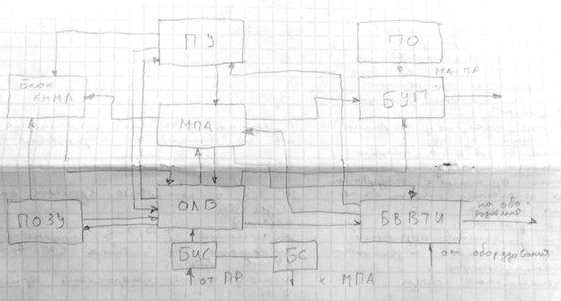
\includegraphics[width=1\linewidth]{Figures/block.png}
    \caption{Функциональная схема аналогового позиционирования манипулятора по одной координате}
    \label{fig:block}
\end{figure}

\begin{figure}[ht]
    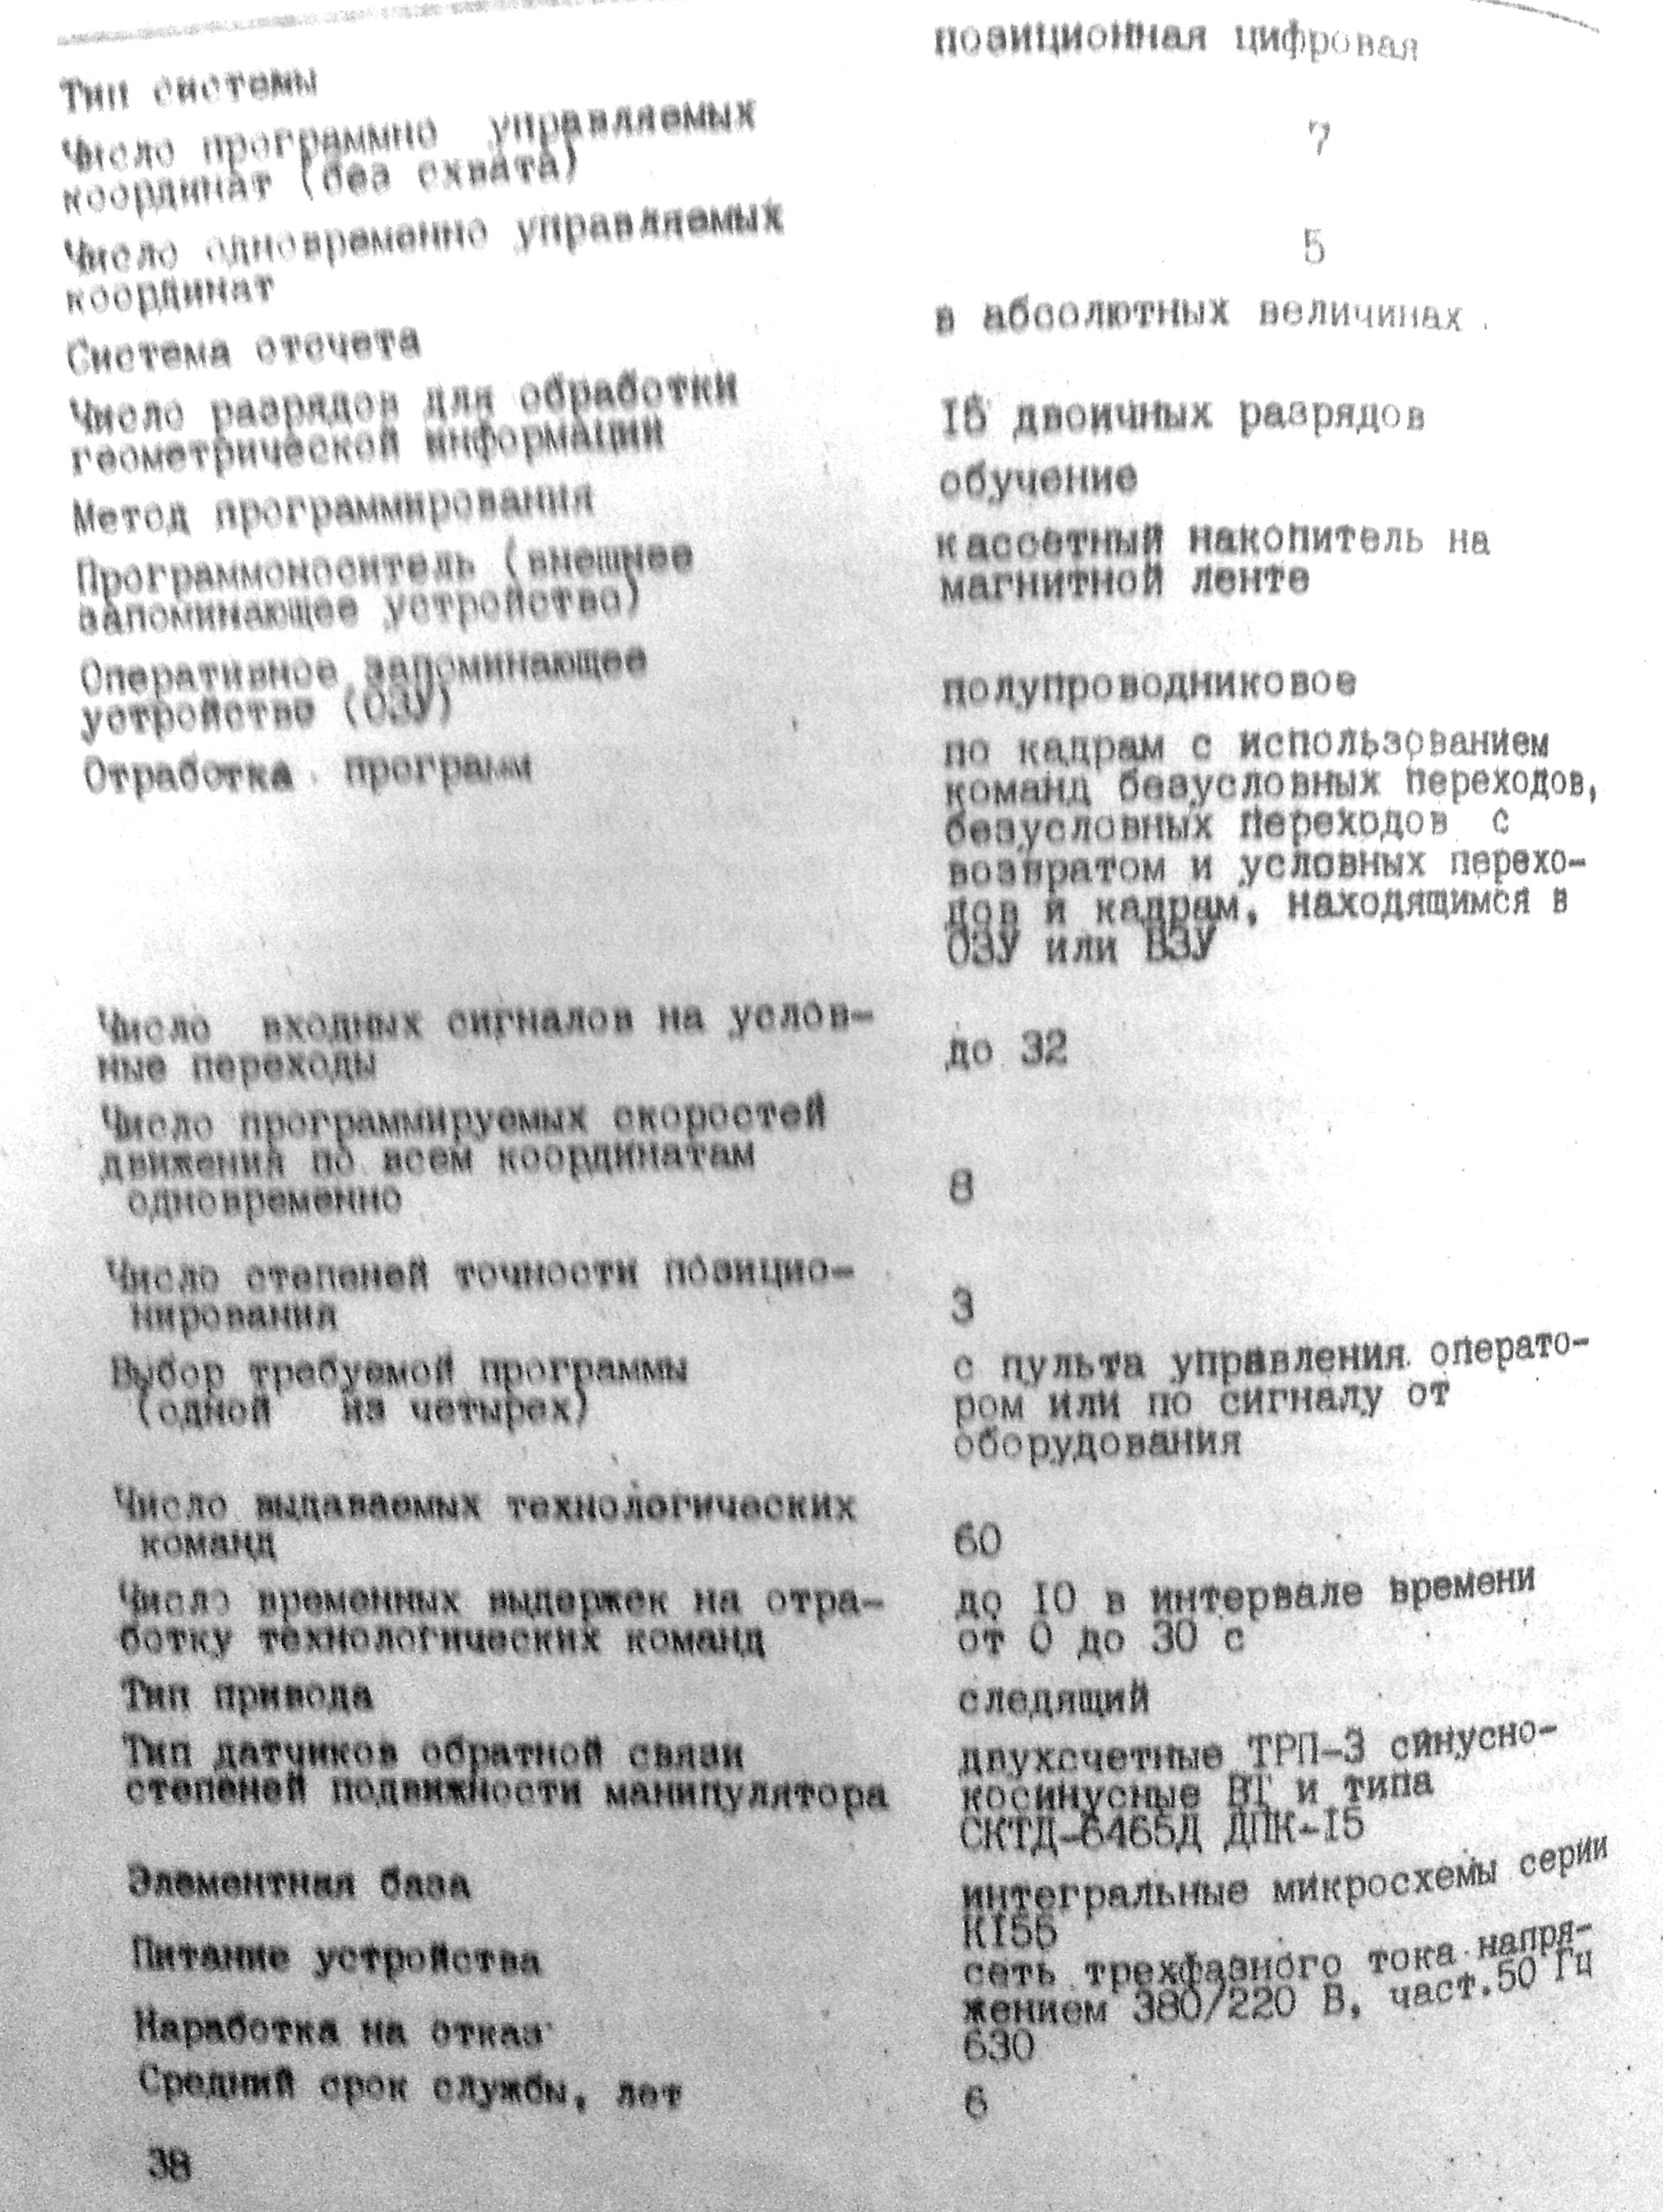
\includegraphics[width=1\linewidth]{Figures/table.png}
    \caption{Основные технические характеристики устройств типа УПМ}
    \label{fig:table}
\end{figure}

МПА работает по жестким ``машинным'' циклам-состояниям; для хранения текущего состояния используется рабочий регистр состояния УРС, новое состояние подготавливается в буферном регистре.

Матрица микропрограммы (ММ) предназначена для формирования управляющих импульсов микроопераций, используемых операционными узлами устройства.

Матрица переходов (МП) - набор логических комбинационных схем И-ИЛИ-НЕ, обеспечивающих формирование нового состояния автомата по результатам анализа входных воздействий, отражающих очередное состояние алгоритма.

Узел контроля осуществляет контроль ОЛБ, БС, ПЧ.
